\section{Komplexität}
	
\begin{frame}{\FrameName}
\begin{itemize}[<+->]
	\item Vertex Cover lässt sich auf SGP reduzieren
	\item Zusammenhang mit Addition Chains \textcolor{gray}{(nicht im Vortrag)}
\end{itemize}
\end{frame}

\begin{frame}{\FrameName}
\begin{block}{Vertex Cover}
	\Gap
	Suche (minimale) Menge von Knoten, sodass jede Kante mindestens einen dieser Knoten enthält.\linebreak
	$ $\linebreak
	
	\only<1>{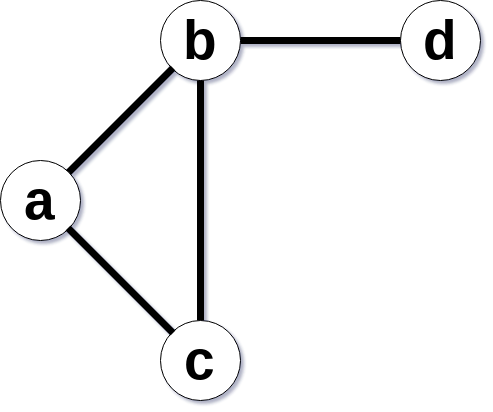
\includegraphics[width=0.25\textwidth]{Images/VertexCover/blank}}
	\only<2>{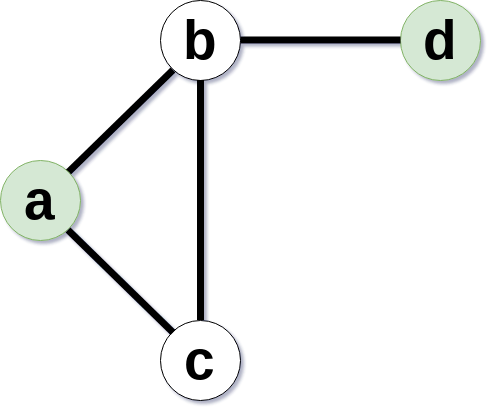
\includegraphics[width=0.25\textwidth]{Images/VertexCover/wrong}}
	\only<3>{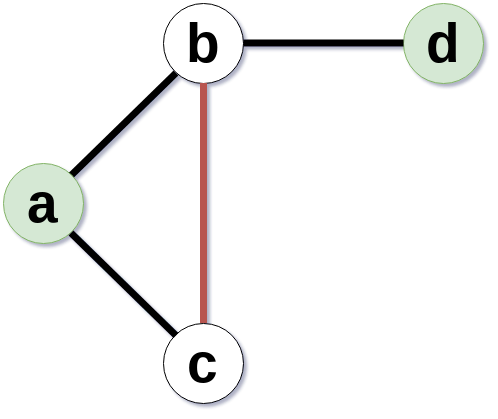
\includegraphics[width=0.25\textwidth]{Images/VertexCover/wrongMarked}}
	\only<4>{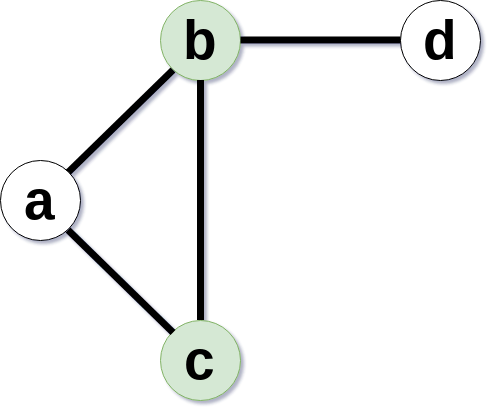
\includegraphics[width=0.25\textwidth]{Images/VertexCover/right}}
	\visible<3>{\alert{(Kein Vertex Cover!)}}
\end{block}
\end{frame}

\newcommand{\ExampleGraphV}{V = \{a,b,c,d\}}
\newcommand{\ExampleGraphE}{E = 
	\begin{Bmatrix}
		\{a,b\},
		\{a,c\},
		\{b,c\},
		\{b,d\}
	\end{Bmatrix}
}

\begin{frame}{\FrameName}
\begin{block}{NP-härte}
	\begin{itemize}[<+->]
			\item Betrachte nur Graphen mit maximalen Knoten-Grad 3
			\item Überführung von Graphen zu Wörtern
			\item Zeige, dass man über die kleinsete Grammatik einen Vertex Cover bestimmen kann
			\item Berechne Upper Bound für effiziente Approximation \linebreak (außer $P=NP$)
		\end{itemize}
\end{block}
\end{frame}

\begin{frame}{\FrameName}
\begin{block}{Beispiel Graph}
	\Gap
	$$\ExampleGraphV$$ 
	$$\ExampleGraphE$$
	\begin{center}
		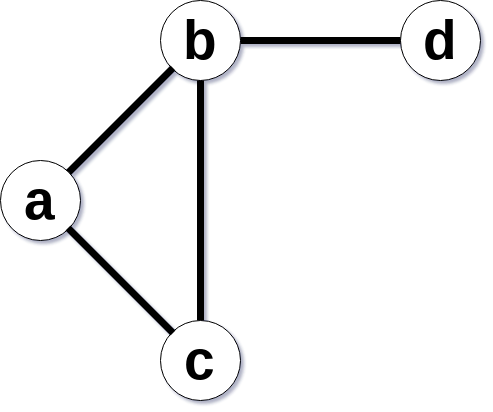
\includegraphics[width=0.35\textwidth]{Images/VertexCover/blank}
	\end{center}
\end{block}
\end{frame}

\newcommand{\ProdRuleOne}[1]{(\# #1 \Fresh #1\#  \Fresh )^2}
\newcommand{\ProdRuleTwo}[1]{\# #1 \#  \Fresh}
\newcommand{\ProdRuleThree}[2]{\# #1 \# #2\#  \Fresh}
\newcommand{\PhantomAlpha}{\phantom{\alpha_{Beispiel} = (}}
\newcommand{\ReductionExample}{
	$
		\alpha_{Beispiel} =
		\textcolor{OrangeRed}{
			\foreach \n in {a,b,c,d}{\ProdRuleOne{\n}}
		} \linebreak
		\PhantomAlpha
		\textcolor{PineGreen}{
			\foreach \n in {a,b,c,d}{\ProdRuleTwo{\n}}
		} \linebreak
		\PhantomAlpha
		\textcolor{RoyalBlue}{
			\ProdRuleThree{a}{b}
			\ProdRuleThree{a}{c}
			\ProdRuleThree{b}{c}
			\ProdRuleThree{b}{d}
		} \linebreak
	$
}

\begin{frame}{\FrameName}
\begin{block}{Graphen zu String überführen}
	\Gap
	$
	\alpha =
	\textcolor{OrangeRed}{
		\prod\limits_{v_i \in V}\ProdRuleOne{v_i}}
	\textcolor{PineGreen}{
		\prod\limits_{v_i \in V}(\ProdRuleTwo{v_i})}
	\textcolor{RoyalBlue}{
			\prod\limits_{\{v_i,v_j\} \in E}(\ProdRuleThree{v_i}{v_j})}
	$

	
	\visible<2>{
		\Gap
			$\ExampleGraphV; \ExampleGraphE$ \newline
		\Gap
		\ReductionExample
	}
\end{block}
\end{frame}

\begin{frame}{\FrameName}
	\ReductionExample
\begin{block}{Eigenschaften der kleinsten Grammatik}
	\begin{itemize}[<+->]
		\item Jedes Nichtterminal expandiert zu $\#v_i$, $v_i\#$ oder $\#v_i\#$
		\item Enthält Regeln der Form $T_j \rightarrow \#v_i$ und $T_j \rightarrow v_i\#$
		\item $C = \{v_i \in V | \exists T_j \rightarrow \#v_i\#\}$ ist (minimale) Vertex Cover
	\end{itemize}
\end{block}
\end{frame}

\begin{frame}{\FrameName}
\begin{block}{Approximation Ratio}
	\begin{itemize}[<+->]
		\item $m^* = 15|V| + 3|E| + |C|$
		\item Es ist ($NP$) hart Vertex Cover kleiner als $\frac{145}{144} \cdot |C|$ zu finden ($\frac{145}{144}\approx 1,006944...$)
		\item $\rho = \frac{15|V| + 3|E| + \frac{145}{144}|C|}{15|V| + 3|E| + |C|}$
		\item $\rho \geq \frac{15|V| + 3 \cdot \frac{3}{2}|V| + \frac{145}{144}(\frac{1}{3}|V|)}{15|V| + 3 \cdot \frac{3}{2}|V| + \frac{1}{3}|V|} = \frac{8569}{8568} \approx 1,0001167...$
	\end{itemize}
\end{block}
\end{frame}